\documentclass{article}
\usepackage[T1]{fontenc}
\usepackage{lmodern}
\usepackage{amsmath}
\usepackage{graphicx}
\usepackage{float}
\usepackage{listings}
\usepackage{xcolor}
\usepackage[polish]{babel}

\usepackage[a4paper, margin=2.54cm]{geometry}

\title{Praca domowa 3\\Porównanie metody gradientowej\\ z symulowanym wyżarzaniem\\
oraz szukaniem przypadkowym}
\author{Damian Jankowski s188597}

\begin{document}

\maketitle

\section{Wstęp}
Celem pracy domowej jest porównanie trzech metod szukania minimum
funkcji: metody gradientowej, symulowanego wyżarzania oraz z szukaniem przypadkowym. 
W tym celu wybrałem funkcję
$f(x, y) = 4x^2+2*y^2-4xy$. Minimum funkcji to $f(0, 0) = 0$.

Poszukiwanie minimum funkcji
zaczęłem od wybrania losowego punktu startowego $X_0$ z zakresu
$-10 \le x \le 10$ oraz $-10 \le y \le 10$.

\begin{figure}[H]
    \centering
    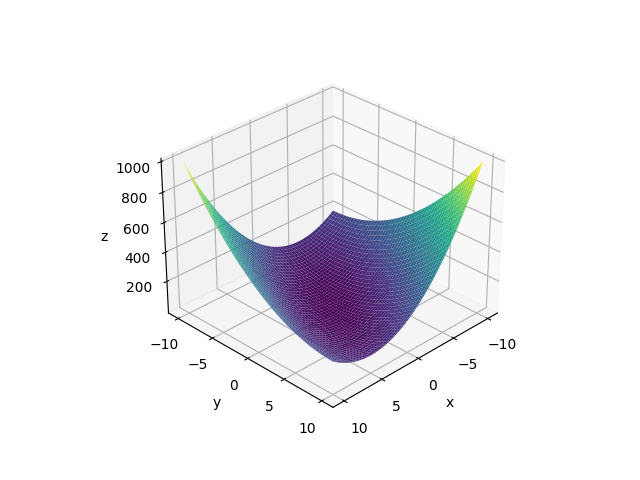
\includegraphics[width=0.5\textwidth]{function.png}
    \caption{Wykres funkcji $f(x, y)$}
\end{figure}

\section{Metoda symulowanego wyżarzania}
Metoda symulowanego wyżarzania polega na losowaniu kolejnych punktów
z pewnego otoczenia punktu $X_k$ i sprawdzaniu czy wartość funkcji
w tym punkcie jest mniejsza niż w poprzednim. Jeśli tak to punkt
$X_{k+1}$ staje się nowym punktem startowym. Jeśli nie to punkt
$X_{k+1}$ jest losowany ponownie. Wraz z kolejnymi iteracjami
otoczenie punktu $X_k$ zmniejsza się. W ten sposób metoda
symulowanego wyżarzania przeszukuje coraz mniejsze obszary
wokół punktu $X_k$.

\subsection{Opis kroków}

\begin{enumerate}
    \item Wybranie losowego punktu startowego $X_0$
    \item Wyznaczenie wartości funkcji $f(X_k)$
    \item Wyznaczenie nowego punktu $w'= w + \Delta w$ z otoczenia punktu $X_k$,
    gdzie $\Delta w$ jest realizacją zmiennej losowej o rozkładzie normalnym
    $g(\Delta w,T) = (2 \pi T) ^{-\frac{n}{2}} e^{-\frac{{\Delta w }^2}{2T}}$
    \item Wyznaczenie wartości funkcji $f(w')$
    \item Podstawienie $w'$ za $w$ jeśli $f(w') < f(w)$ lub gdy
    $r < \frac{1}{1 + e^{\frac{\Delta f}{T}}}$, gdzie $r$ jest realizacją zmiennej
    losowej o rozkładzie jednostajnym na przedziale $[0, 1]$
    \item Zmniejszenie temperatury $T' = \alpha T$
    \item Zwiększenie licznika iteracji $k = k + 1$. Zakończenie gdy $k = k_{max}$ lub gdy $f(X_k) < f_{min}$
\end{enumerate}

\section{Metoda szukania przypadkowego}
Metoda szukania przypadkowego podobnie jak metoda symulowanego
wyżarzania polega na losowaniu kolejnych punktów z pewnego
otoczenia punktu $X_k$. W tym przypadku zakres losowania
jest stały i nie zmniejsza się wraz z kolejnymi iteracjami.

\subsection{Opis kroków}

\begin{enumerate}
    \item Wybranie losowego punktu startowego $X_0$
    \item Wyznaczenie wartości funkcji $f(X_k)$
    \item Wyznaczenie nowego punktu $w'= w + \Delta w$ z otoczenia punktu $X_k$,
    gdzie $\Delta w$ jest realizacją zmiennej losowej o rozkładzie normalnym
    $g(\Delta w,\sigma) = (2 \pi \sigma) ^{-\frac{n}{2}} e^{-\frac{{\Delta w }^2}{2\sigma}}$
    (w tym przypadku $\sigma = const$)
    \item Wyznaczenie wartości funkcji $f(w')$
    \item Podstawienie $w'$ za $w$ jeśli $f(w') < f(w)$ 
    \item Zwiększenie licznika iteracji $k = k + 1$. Zakończenie gdy $k = k_{max}$ lub gdy $f(X_k) < f_{min}$
\end{enumerate}

\section{Zadanie}

W przypadku symulowanego wyżarzania przyjąłem:
\begin{itemize}
    \item $T_0 = 10$
    \item $\alpha = 0.99$
\end{itemize}

Natomiast dla metody szukania przypadkowego:
\begin{itemize}
    \item $\sigma = 0.1$
\end{itemize}

Wszystkie 3 metody kończyły się gdy wartość funkcji w punkcie $X_k$
była mniejsza niż $f_{min} = 10^{-4}$ lub gdy liczba iteracji
osiągnęła wartość $k_{max} = 10000$.

Symulację przeprowadziłem dla 1000 losowo wybranych punktów startowych.
Średnia liczba iteracji potrzebna do osiągnięcia wartości funkcji
mniejszej niż $f_{min}$ wyniosła:

\begin{itemize}
    \item Metoda gradientowa:  34.729
    \item Metoda symulowanego wyżarzania:  764.728
    \item Metoda szukania przypadkowego:  647.866
\end{itemize}

\begin{figure}[H]
    \centering
    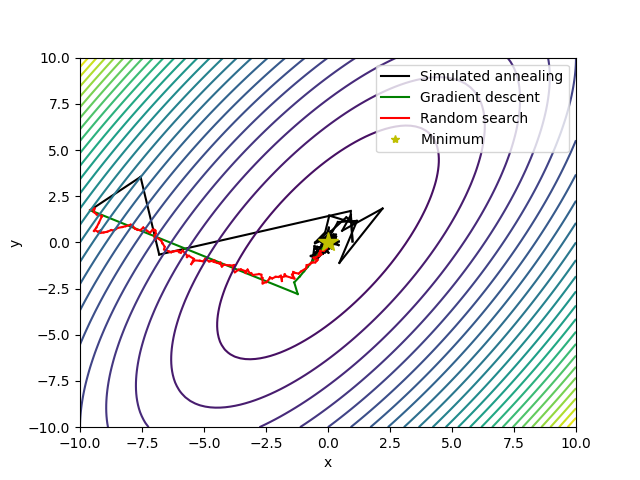
\includegraphics[width=0.5\textwidth]{plot.png}
    \caption{Rzut 2D funkcji $f(x, y)$ oraz kolejne kroki
    minimalizacji metodą gradientową,} {z wyżarzaniem oraz 
    z szukaniem przypadkowym}
\end{figure}

\section{Wnioski}
Wyniki symulacji pokazują, że metoda gradientowa jest znacznie
szybsza od pozostałych metod. Metoda symulowanego wyżarzania
potrzebowała średnio 22 razy więcej iteracji niż metoda gradientowa.

W porównaniu metod gradientowych, wyżarzania oraz szukania 
przypadkowego można wyróżnić kilka wniosków:

Metoda gradientowa jest najskuteczniejsza, gdyż pozwala na znalezienie 
globalnego minimum, jeśli funkcja jest różniczkowalna i nie ma zbyt 
wiele minimów lokalnych. Metoda ta działa dobrze dla prostych funkcji, 
ale może mieć problemy z funkcjami nieliniowymi, 
gdzie minimum globalne znajduje się w dolinie.

Metoda wyżarzania jest skuteczna, ale wymaga więcej czasu niż metoda 
gradientowa. W przeciwieństwie do metody gradientowej, metoda 
wyżarzania nie zawsze znajduje globalne minimum, ale może znaleźć 
rozwiązanie optymalne dla funkcji, które mają wiele minimów lokalnych. 
Metoda ta działa dobrze, jeśli funkcja jest nieregularna i ma wiele 
lokalnych minimów.

Metoda szukania przypadkowego jest najmniej skuteczna, ale jest najprostsza do 
zastosowania. Ta metoda działa dobrze dla funkcji, które mają wiele 
minimów lokalnych, ale może trwać bardzo długo, zanim znajdzie się 
globalne minimum. W rzeczywistości, jeśli funkcja ma więcej niż 
kilka wymiarów, szansa na znalezienie globalnego minimum jest bardzo niska.
W związku z powyższymi wnioskami, wybór odpowiedniej metody optymalizacji 
zależy od charakterystyki funkcji, której minimum poszukujemy, 
a także od czasu, jaki mamy na wykonanie obliczeń. 

W przypadku, gdy mamy do czynienia z 
funkcjami nieregularnymi i wieloma minimami lokalnymi, 
a czas nie jest czynnikiem decydującym, zaleca się zastosowanie 
metody wyżarzania. Natomiast, gdy czas jest ważny, a funkcja jest 
różniczkowalna i nie ma wielu minimów lokalnych, najlepiej wykorzystać 
metodę gradientową. 

Metoda szukania przypadkowego może być przydatna, 
gdy mamy do czynienia z funkcją, która ma wiele minimów lokalnych, ale 
nie jest to zalecane dla złożonych funkcji wielowymiarowych.

\section{Kod programu}
\lstinputlisting[
language=python,  
basicstyle=\small\tt,
keywordstyle=\color{blue},
backgroundcolor=\color{cyan!10}
]{main.py}

\end{document}
